% ===== AGRADECIMIENTOS (solo main-uis.tex) =====
\chapter*{Agradecimientos}
\markboth{Agradecimientos}{Agradecimientos}

\lettrine[lines=2]{A}{gradecido} de forma inconmensurable con Dios, nuestro SEÑOR, por concebirme como criatura suya y hacerme parte de su magna creación. Maravillado estoy con la majestuosidad, elegancia, detalle, simplicidad, armonía, entre otras excelsas cualidades de la creación que Dios erigió como morada de sus criaturas y que parcialmente ha mostrado frente a mis ojos. Cada aspecto de la naturaleza el Señor con tanto cuidado lo pensó, y con la más infinita maestría lo ejecutó, y acá estamos ante el majestuoso sistema del mundo que el arquitecto universal erigió y por el cual su gloria es manifiesta, pues no hay lugar en la tierra o en las regiones supralunares donde tu gloria no sea manifiesta. Glorioso te muestras en la escala de las galaxias, dichoso te muestras en el átomo y tus procesos; todo lo dotaste de tanta vida, riqueza para comunicarse y cierto misterio que hace única cada cosa. Este mundo es magno, grande, lleno de gloria y obedece a tu palabra, que en el principio del mundo pronunciaste para que todo se crease y avanzara en armonía hacia tus propósitos. Nos lo entregaste a nosotros para su cuidado y como materia prima para nuestras creaciones, porque como creadores nos concebiste, pues nos hiciste a tu imagen y semejanza. Un mundo nos entregaste y un mundo te entregaremos, y DIOS, como agradecimiento por haberme creado y darme siempre salud y gran vitalidad en toda mi vida, me comprometo a hacer lo que en mí esté para pulir la tierra en la que habito. Y no solo mi compromiso es con la tierra que carece de tu aliento vital, sino también con tus hijos, pues en cuanto a mí esté, elevaré los espíritus de quienes hagan parte de mi camino hacia la verdad, lo bello y, en suma, lo que es correcto y bueno.

Gracias le doy a nuestro SEÑOR por mostrarme varios de los misterios de la naturaleza e iniciarme en ellos; gracias por hacerme parte de esta maravillosa creación, y aún más agradecido por no concebir el universo sin mi alma en él. Gracias por tenerme en tus propósitos, y gracias por mostrarme caminos dignos de seguir.

Agradezco a la humanidad por haber reconocido en la ciencia un instrumento para encontrar la verdad y mostrarle a todo el mundo la gloria de la creación; gracias por haberle puesto nombre y sistema a la filosofía de la naturaleza, gracias por la lengua que me enseñaron para comunicarme con mis contemporáneos y posiblemente con las generaciones venideras.

Quiero agradecer por darme una madre que siempre cuidó bien de mí, quiso lo mejor para mí y me apoyó mientras encontraba la manera de defenderme en este mundo y encontrar por mí mismo el sustento.

Gracias quiero dar al programa Generación E: Excelencia del Estado Colombiano, que me ayudó en mi sustento; sin dicho apoyo hubiese sido muy difícil haber concluido mis estudios. Por tanto, doy gracias y espero que siempre se apoye, y con el tiempo en mayor medida, el talento nacional y el buen encaminamiento de los jóvenes.

Esto es: gracias, Dios, por concebirme como hijo tuyo; gracias por darme una muy buena madre; gracias por darme el lenguaje y cierta inteligencia para entender algunos fenómenos de la naturaleza; gracias por el apoyo y las oportunidades, las que ya han pasado y todas las que vendrán.

\bigskip

\begin{center}
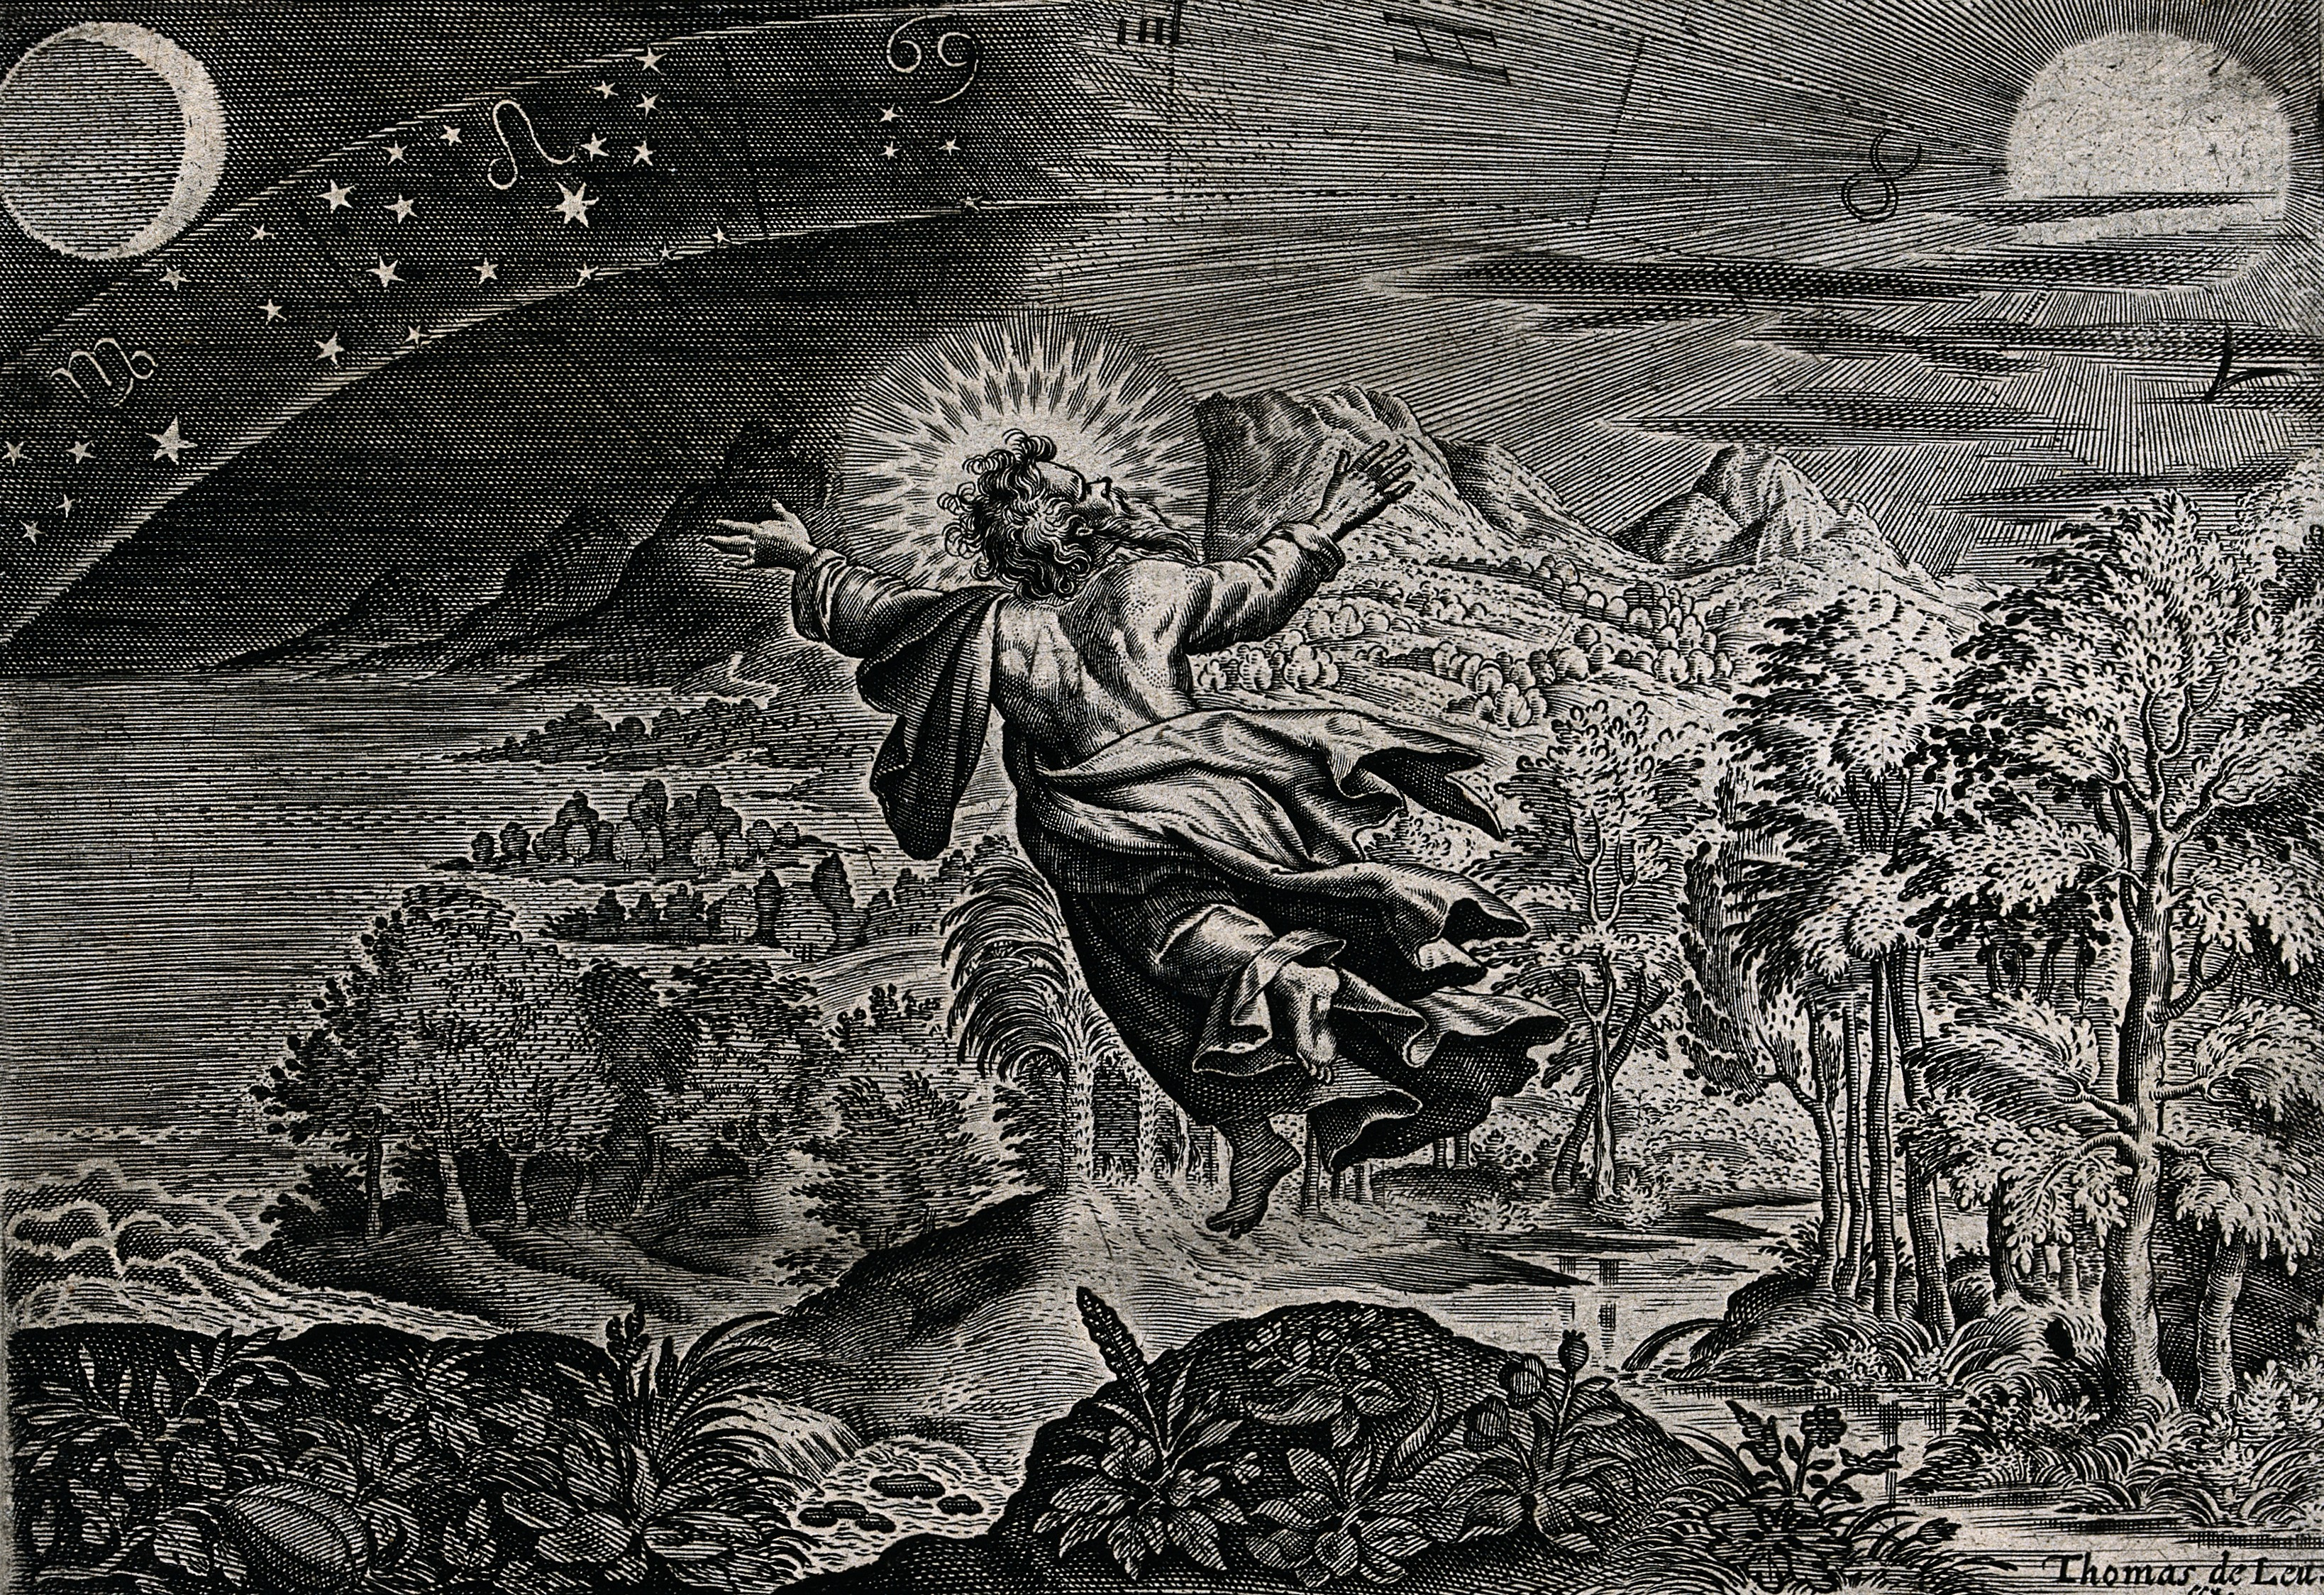
\includegraphics[width=0.7\textwidth]{figures/god_creates_sun_moon_stars.jpg}

{\small\itshape God creates the sun, moon and stars. Thomas de Leu. (1600).}

\vspace{0.7cm}
\textsc{Solo tú, Dios, eres la verdad, y a tu gloria consagro mi vida.}
\end{center}

\medskip

\begin{flushright}
\textsc{Tu humilde y sincero siervo,}\\[0.7em]
\textit{Jhonatan S. Blanco.}
\end{flushright}

\clearpage
